\section{Graphical User Interface}

Like other subsystems, the GUI core is designed to be platform
independent. Therefore only the \emph{outermost} shell contains toolkit
specific code.

\subsection{Architecture}

The GUI is modeled after the Model-View-ViewModel architecture. The
\emph{Model} represents the underlying data structures and business
logic. It is provided by the generated classes from the actual
datamodel. 

\emph{View Models} provide
display specific functionality like formatting, transient state holding
and implementing the user's possible actions. They always inherit from
\emph{Kistl.Client.Presentables.ViewModel}.
Common implementations reside in the
\emph{Kistl.Client.Presentables} namespace.

\emph{Control Kinds} are representing a way how \emph{ViewModels} would like to be displayed. For example:

\begin{itemize}
\item as a TextBox
\item as a DropDownList
\item as a CheckBox
\item as a RadioButtonList
\end{itemize}

\emph{Control Kinds} are simply a sort of enumeration items. They do not provide any services. 
\emph{ControlKinds} can be put into a hierarchy. That enables the infrastructure to choose another view if a certian 
\emph{ControlKind} is not implemented in a Toolkit.
 
Finally,
\emph{Views} (editors and displays) are the actual components taking
care of showing content to the user and converting the users keypresses
and clicks into calls on the view models interface.  Views are
toolkit\footnote{Toolkits are GUI libraries like WPF, GTK\# or Windows
Forms but can also be implemented by more complex providers such as
ASP.NET.} specific and reside in the toolkit's respective assembly.

This architecture decouples the actual functionality of the Model and
the View Model completly from the inner workings of a toolkit and
thereby maximise the reuse of code between different clients.

\begin{figure}[ht]
	\begin{center}
		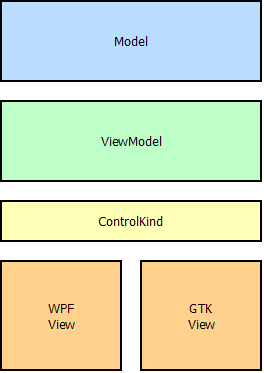
\includegraphics[width=0.6\textwidth]{images/GUI_Relation_MVVM.png}
		\caption{Relation of Models, ViewModels, ControlKinds and Views}
		\label{GUI_Relation_MVVM}
	\end{center}
\end{figure}

\subsection{Plumbing}

The three layers are connected through two sets of descriptors and \emph{ControlKinds}. The
\emph{ViewModelDescriptor}s contain information about the
available View Models and their preferred way of being displayed. 

\begin{CS}
public interface ViewModelDescriptor
{
	Kistl.App.GUI.ControlKind DefaultKind;
	Kistl.App.GUI.ControlKind DefaultDisplayKind;
	Kistl.App.GUI.ControlKind DefaultGridCellDisplayKind;
	Kistl.App.GUI.ControlKind DefaultGridCellKind;
	
	string Description;
	
	Kistl.App.Base.TypeRef ViewModelRef;
}
\end{CS}

\emph{ViewDescriptor}s contain information about controls which are capable of displaying certian \emph{ControlKinds}.

\begin{CS}
public interface ViewModelDescriptor
{
	Kistl.App.GUI.ControlKind ControlKind;
	Kistl.App.Base.TypeRef ControlRef;
	Kistl.App.GUI.Toolkit Toolkit;
}
\end{CS}

\subsubsection{Some implemented ViewModels}

\begin{description}

\item[\emph{DataObjectViewModel}]{represent a complete data object;
provide standardised access to properties; provide non-standard ViewModels
with additional functionality; selected via
\emph{ObjectClass.DefaultViewModelDescriptor}}

\item[\emph{BaseValueViewModel}s]{represent a specific piece of simple data (strings, DateTimes);
Data can be the a Propertiy, MethodResults or simply a Value; Properties and Parameter of Methods selects their \emph{ViewModel} via their
\emph{ValueModelDescriptor} Property; }

\item[ActionViewModel]{represent a Method which can be invoked in the UI.}

\item[ObjectEditor.WorkspaceViewModel] { This ViewModel implements all featurs of and Object Editor. This includes Cancel, Save or selecting the current item.}

\end{description} 

\subsubsection{Control Kind}

The \emph{ControlKind} specifies the toolkit-independent kind or type of
control that should display a given Presentable. While the View
specifies the Control Kind it implements the Presentable requests a
specific Kind to be displayed via the
\emph{PresentableModelDescriptor.DefaultControlKind} value.

In special situations this default value can be overridden. For example,
the metadata of a property contains a \emph{RequestedControlKind} which
is used instead of the \emph{DefaultControlKind} when present. If there
is no View matching the requested Kind, the infrastructure may either
fall back to the default control kind, or use a similar control kind
from higher up in the hierarchy.

Typical kinds of controls:

\begin{description}

\item[WorkspaceWindow] {the top-level control within which all user
interaction happens}

\item[SelectionTaskDialog] {a dialog letting the user select something
from a longer list of items}

\item[ObjectView] {display the modeled object in full}

\item[ObjectListEntry] {display the modeled object as item in a list}

\item[TextEntry] {lets the user edit a property as text}

\item[IntegerSlider] {lets the user edit a number with a slider}

\item[YesNoCheckbox] {a simple yes/no checkbox}

\item[YesNoOtherText] {radio buttons allowing one to select either "yes",
"no" or a TextEntry field}

\item[ExtendedYesNoCheckbox] {a checkbox with additional text as label}

\end{description}

The kind of a control is identified by the \emph{ControlKind}'s class. The
hierarchy between different kinds of controls is modeled with inheritance.

\subsubsection{Views}

Their descriptors list the available Views by Toolkit and which ControlKind they represent. \emph{View Descriptors} can define which \emph{ViewModel}s (or Interfaces to ViewModels) are supported.

\subsection{Resolving ViewModels}

\emph{ViewModels} are resolved by the \emph{IViewModelFactory}

\begin{CS}
public interface IViewModelFactory
{
    void ShowModel(ViewModel mdl, bool activate);
    void ShowModel(ViewModel mdl, Kistl.App.GUI.ControlKind kind, bool activate);

    void CreateTimer(TimeSpan tickLength, Action action);
    string GetSourceFileNameFromUser(params string[] filter);
    string GetDestinationFileNameFromUser(string filename, params string[] filter);
    Toolkit Toolkit { get; }

    // Create Models
    TModelFactory CreateViewModel<TModelFactory>() where TModelFactory : class;
    TModelFactory CreateViewModel<TModelFactory>(Kistl.API.IDataObject obj) where TModelFactory : class;
    TModelFactory CreateViewModel<TModelFactory>(Kistl.API.ICompoundObject obj) where TModelFactory : class;
    TModelFactory CreateViewModel<TModelFactory>(Kistl.App.Base.Property p) where TModelFactory : class;
    TModelFactory CreateViewModel<TModelFactory>(Kistl.App.Base.BaseParameter p) where TModelFactory : class;
    TModelFactory CreateViewModel<TModelFactory>(Kistl.App.Base.Method m) where TModelFactory : class;
    TModelFactory CreateViewModel<TModelFactory>(System.Type t) where TModelFactory : class;

    // IMultipleInstancesManager
    void OnIMultipleInstancesManagerCreated(Kistl.API.IKistlContext ctx, IMultipleInstancesManager workspace);
    void OnIMultipleInstancesManagerDisposed(Kistl.API.IKistlContext ctx, IMultipleInstancesManager workspace);
}
\end{CS}

\emph{ViewModel}s can be created directly if the requested \emph{ViewModel} is
known. Some \emph{ObjectClasses} (ObjectClass, Property, Method, Parameter,
etc.) can declare a more specific \emph{ViewModel}. Use a more specific
\emph{CreateViewModel} overload in such a case.

The most obvious example is \emph{Property}. There is a need for different
\emph{ViewModel}s for a \emph{StringProperty} vs.
\emph{ObjectReferenceProperty}. Each \emph{ViewModel} for displaying Properties
derives from a very basic \emph{BaseValueViewModel}.

\begin{description}
\item[IntProperty] { is displayed by a NullableStructValueViewModel of type int
}
\item[BoolProperty] { is displayed by a NullableStructValueViewModel of type
bool}
\item[DecimalProperty] { is displayed by a NullableStructValueViewModel of type
decimal }
\item[String\-Property] { is displayed by a ClassValue\-ViewModel of type string
or MultiLine\-StringValue\-View\-Model }
\item[DateTimeProperty] { is displayed by a NullableDateTimePropertyViewModel }
\item[ObjectReference\-Property] { is displayed by a
Object\-Reference\-ViewModel, Object\-Collection\-ViewModel or Object\-List\-ViewModel }
\end{description}

Create a specific \emph{ViewModel} by calling:

\begin{CS}
	mdlFactory.CreateViewModel<WorkspaceViewModel.Factory>().Invoke(ctx);
\end{CS}

Create a \emph{ViewModel} for a \emph{Property} by calling:

\begin{CS}
	ViewModelFactory.CreateViewModel<BaseValueViewModel.Factory>(prop).Invoke(DataContext,
prop.GetValueModel(Object));
\end{CS}

Create a \emph{ViewModel} for a \emph{IDataObject} by calling:

\begin{CS}
	ViewModelFactory.CreateViewModel<DataObjectViewModel.Factory>(obj).Invoke(DataContext, obj);
\end{CS}

The \emph{ViewModelFactory} will look up the \emph{IDataObject}s type and tries
to find it's \emph{ObjectClass}. Then it looks up the \emph{ViewModelDescriptor}
and creates the \emph{ViewModel}.

\subsection{Implementation}

\subsubsection{Implementing a ViewModel}

\subsubsection{Implementing a WPF View}

\subsection{Asynchronous Loading}

\emph{Not yet implemented.}

To facilitate low-latency user interfaces, the ViewModels should implement a
thin proxy layer to delegate all potential blocking operations onto a worker
thread. To keep programming this layer easy, there are a few helper classes and
a few constraints on the available interface mechanisms as well as a consistent
contract over all compliant ViewModels.

There are only three ways to communicate over the \emph{thread gap}:
\begin{enumerate}
\item{accessing a property}
\item{calling a \emph{void} function (with not \emph{out} or \emph{ref} parameters)}
\item{having an \emph{EventHandler} called}
\end{enumerate}

All compliant ViewModels provide a \emph{IsLoading} property that signifies
whether any background processing is active. While this property is true, any
value read from a property may be stale and/or about to be replaced. Changes to
the visible value of a property are always reported via the
\emph{PropertyChanged} event from the \emph{INotifyPropertyChanged} interface.
This should suffice for enabling binding frameworks to show current values to
the user: When reading a value from a property, a cached value is returned
immediately and optionally a refresh is triggered, which in turn may cause a
PropertyChanged event a little bit later.

In the case of time-dependent values, the ViewModel has to take care
to establish a periodic refresh timer\footnote{Todo: such a timer should be
provided by the infrastructure for platform dependent refreshing} which
triggers PropertyChanged events when new values arrive.

Similarily, methods called on the ViewModel do not actually do their work
immediately, but delegate to the background worker thread. Results either show
up automatically through changed properties and the PropertyChanged event or
via specialized events.

\subsubsection{Thread Safety}

The ViewModel is designed to be accessed from a single UI thread. Due to the
low latency of the public interface, this should pose no problem. The ViewModel
internally takes care of all synchronization with the worker thread. Due to the
asynchronicity of the underlying data it is quite possible that the values of
properties change while a method on the UI thread is currently executing.

\subsubsection{Automatic Generation}

Due to the restricted set of operations allowed, the proxy can and should be
automatically generated, freeing the ViewModel from the intricacies of
synchronizing and delegating across thread boundaries. Special needs like
callback parameters and time-dependent values have to be communicated via
special Attributes.

